\chapter{Fractions de polynômes}

\section{Rappels numériques}
Une fraction représente une partie d'un objet ou d'une quantité, par exemple une part de gâteau, une partie d'un champ, etc.

Pour pouvoir additionner ou soustraire deux quantités, il est nécessaire qu'elles aient la même signification. Par exemple, je ne peux pas juste mettre ensemble une moitié de gâteau et un tiers du même gâteau. Je vais devoir trouver une unité commune. Dans cet exemple de gâteau, si je divise ma moitié en trois, j'ai trois sixièmes de gâteau et mon tiers en deux, deux sixièmes. Ainsi en tout j'ai cinq sixièmes du gâteau. Pour parler plus simplement, une petite précision de nomenclature est nécessaire :

\begin{definition}
Pour une fraction du type
$$
\frac{a}{b},
$$
$a$ est appelé le \emph{numérateur} (il sert à compter le nombre de parties) et $b$ le \emph{dénominateur} (il indique de quelle type de partie il s'agit)
\end{definition}

Certaines fractions peuvent être expliquées plus simplement. Par exemple deux quarts de gâteau représentent une moitié. Dans un cadre plus général, on peut \emph{simplifier une fraction} si le numérateur et le dénominateur peuvent être divisés par le même nombre.

Comme nous l'avons vu dans l'exemple précédent, pour additionner ou soustraire deux fractions, il faut trouver un dénominateur commun. Bien sûr, nous pouvons toujours prendre la multiplication des dénominateurs, mais les fractions ainsi obtenues sont souvent trop compliquées et demandent alors une simplification. Pour ne pas faire le travail à double, nous allons plutôt prendre le PPMC des numérateurs.

\begin{exemple}
Additionner les deux fractions suivantes :
$$
\frac{3}{20} + \frac{7}{50}.
$$
Il nous faut donc trouver le PPMC de $20$ et $50$. On cherche donc à exprimer $20$ et $50$ en produits de nombres premier :
$$
\begin{array}{lcl}
20 &=& 2^2 \cdot 5 \\
50 &=& 2 \cdot 5^2
\end{array}
$$
Ainsi le PPMC est donné par $2^2\cdot 5^2 = 100$. On amplifie la première fraction par $5$ et la seconde par $2$ :
$$
\frac{3\cdot 5}{20 \cdot 5} + \frac{7 \cdot 2}{50 \cdot 2} = \frac{15}{100} + \frac{14}{100} = \frac{15 +14}{100} = \frac{29}{100}.
$$
\end{exemple}

\section{PPMC de polynômes}

Pour les fractions de polynômes, le processus ne change pas. Ainsi il nous faut une méthode pour déterminer le PPMC de deux polynômes.

\begin{enumerate}\index{polynôme!PPMC}
\item Factoriser chaque polynôme
\item Prendre chaque partie de factorisation avec sa plus haute puissance, mais une seule fois
\end{enumerate}

\begin{exemple}\label{PPMC}
Trouver le PPMC de
$$
2x^2 +8x + 8 \mbox{ et } 3x^2 + 15x + 18.
$$
Ainsi
\begin{enumerate}
\item On commence par factoriser chaque polynôme
$$
\begin{array}{lcl}
2x^2 +8x + 8 &=& 2(x+2)^2\\
3x^2 + 15x + 18 &=& 3(x+2)(x+3)
\end{array}
$$
\item Le PPMC est donc donné par 
$$
6(x+2)^2 (x+3)
$$
car $6$ et le PPCM de $3$ et $2$, $(x+2)$ apparaît à la puissance $2$ et  $(x+3)$ apparaît une fois.
\end{enumerate}
\end{exemple}

\section{Simplifier une fraction de polynômes}

Pour simplifier une fraction de polynômes, il faut, comme pour les nombres, trouver ce par quoi l'on peut diviser le numérateur et le dénominateur. Pour les nombres, c'est assez simple, mais pour les polynômes, trouver de tête les diviseurs est plus complexe. Il faut ainsi commencer par factoriser le numérateur et le dénominateur avant de simplifier.

\begin{exemple}
Simplifier
$$
\frac{2x^2 +8x + 8}{6x^2 + 30x + 36}
$$
On factorise numérateur et dénominateur :
$$
\begin{array}{lcl}
2x^2 +8x + 8 &=& 2(x+2)^2\\
6x^2 + 30x + 36 &=& 6(x+2)(x+3)
\end{array}
$$
On remplace ensuite le numérateur et le dénominateur dans la fraction de base :
$$
\frac{2(x+2)^2}{6(x+2)(x+3)} = 
\frac{\xout{2}^1(x+2)^2}{\xout{6}_3(x+2)(x+3)} =
\frac{(x+2)^\xout{2}}{3\xout{(x+2)}(x+3)} =
\frac{(x+2)}{3(x+3)}
$$
\end{exemple}

\section{Additionner deux fractions}

Comme dit précédemment, pour additionner deux polynômes il faut trouver le PPMC des dénominateurs. Cependant dans certains cas, il vaut mieux simplifier d'abord chaque fraction pour éviter des calculs par la suite. Ainsi pour additionner deux fractions de polynômes ;
\begin{enumerate}
\item Simplifier chaque fraction
\item Déterminer le PPMC des dénominateurs
\item Amplifier chaque fraction par ce qu'il manque au dénominateur par rapport au PPMC
\item Additionner les numérateurs et réduire le numérateur
\item Simplifier la fraction
\end{enumerate}

\begin{exemple}
Additionner les fractions
$$
\frac{3}{2x^2 +8x + 8} + \frac{5}{3x^2 + 15x + 18}
$$
\begin{enumerate}
\item Aucune des deux fractions n'est simplifiable
\item Comme dans l'exemple~\ref{PPMC}, il est donné par $6(x+2)^2 (x+3)$
\item On amplifie la première fraction par $\textcolor{red}{3(x+3)}$ et la seconde par $\textcolor{blue}{2(x+2)}$. Ainsi
$$
\begin{array}{l}
\frac{3 \cdot  \textcolor{red}{3(x+3)}}{2(x+2)^2 \cdot  \textcolor{red}{3(x+3)}} + \frac{5\cdot  \textcolor{blue}{2(x+2)}}{3(x+2)(x+3) \cdot \textcolor{blue}{2(x+2)}}
=\\
\\
\frac{9x+27}{6(x+2)^2 (x+3)} + \frac{10x + 20}{6(x+2)^2 (x+3)}
\end{array}
$$
\item On additionne les numérateurs puisque les deux fractions ont le même dénominateur et on réduit :
$$
\frac{9x+27 + 10x + 20}{6(x+2)^2 (x+3)} = \frac{19x + 47}{6(x+2)^2 (x+3)}
$$
\item La fraction obtenue ne peut être simplifiée.
\end{enumerate}
\end{exemple}

\section{Multiplier deux fractions}

Contrairement à ce qu'on pourrait croire, multiplier deux fractions est plus simple que d'en additionner deux. Cependant il ne faut pas confondre les deux méthodes.
\begin{enumerate}
\item Factoriser chaque numérateur et chaque dénominateur
\item Simplifier les polynômes qui apparaissent en haut et en bas (en vertical mais aussi en diagonal)
\item Multiplier les numérateurs entre eux et les dénominateurs entre eux
\end{enumerate}

Attention : il n'y a pas de recherche de PPMC dans la multiplication !

\begin{exemple}
Multiplier 
$$
\frac{18}{2x^2 +8x + 8} \cdot \frac{3x^2 + 15x + 18}{x+3}
$$
Ainsi en suivant la méthode :
\begin{enumerate}
\item On factorise chaque terme :
$$
\frac{18}{2(x+2)^2} \cdot \frac{3(x+2)(x+3)}{x+3}
$$
\item On simplifie :
$$
\frac{\xout{18}^9}{\xout{2}_1(x+2)^2} \cdot \frac{3(x+2)\xout{(x+3)}}{\xout{(x+3)}} = \frac{9}{(x+2)^\xout{2}} \cdot \frac{3\xout{(x+2)}}{1} = 
\frac{9}{(x+2)} \cdot \frac{3}{1}
$$
\item Et on finit par multiplier
$$
\frac{9\cdot 3}{(x+2) \cdot 1} = \frac{27}{(x+2)}
$$
\end{enumerate}
\end{exemple}

\section{Exercices}

\begin{exercice}
Simplifier les fractions suivantes : 
\begin{multicols}{2}
\begin{enumerate}
\item $$\frac{14{{b}^{4}}x\cdot 5ay}{15{{a}^{2}}x\cdot 7{{b}^{3}}y}$$
\item $$\frac{axy-bxy}{ab-{{b}^{2}}}$$
\item $$\frac{a-3}{2{{a}^{2}}-18}$$
\item $$\frac{9{{a}^{5}}-16a}{6{{a}^{2}}{{b}^{2}}-8{{b}^{2}}}$$
\item $$\frac{{{a}^{3}}+{{b}^{3}}}{{{(a-b)}^{2}}+ab}$$
\item $$\frac{4{{(x+y)}^{2}}}{3({{x}^{2}}-{{y}^{2}})}$$
\item $$\frac{{{x}^{2}}-4x+4}{{{x}^{2}}-4}$$
\item $$\frac{8{{a}^{3}}+1}{64{{a}^{6}}-1}$$
\item $$\frac{25{{x}^{2}}+20ax+4{{a}^{2}}}{2(25a{{x}^{3}}-4{{a}^{3}}x)}$$
\item $$\frac{12a{{x}^{2}}+3ax}{8{{x}^{2}}+22x+5}$$
\item $$\frac{{{x}^{2}}-7x-8}{{{x}^{3}}+3{{x}^{2}}+2x}$$
\item $$\frac{8{{x}^{2}}+22x-6}{4{{x}^{2}}+27x-7}$$
\item $$\frac{2{{x}^{2}}-9x+7}{12{{x}^{2}}-21x+9}$$
\item $$\frac{40{{x}^{3}}-5}{12{{x}^{2}}+6x+3}$$
\item $$\frac{{{(a+b)}^{2}}({{a}^{3}}-{{b}^{3}})}{{{({{a}^{2}}-{{b}^{2}})}^{2}}}$$
\item $$\frac{{{x}^{3}}-{{x}^{2}}-4x+4}{{{x}^{2}}-3x+2}$$
\item $$\frac{2{{x}^{3}}+5{{x}^{2}}+4x+1}{{{x}^{3}}+3{{x}^{2}}+3x+1}$$
\item $$\frac{{{x}^{3}}-9{{x}^{2}}+11x+21}{{{x}^{4}}-{{x}^{3}}-4{{x}^{2}}-5x-3}$$
\item $$\frac{{{x}^{4}}-2{{x}^{2}}+1}{3{{x}^{5}}-10{{x}^{3}}+15x-8}$$
\item $$\frac{1+{{x}^{3}}}{1+2x+2{{x}^{2}}+{{x}^{3}}}$$
\item $$\frac{2{{x}^{3}}-7{{x}^{2}}+2x+3}{2{{x}^{3}}-9{{x}^{2}}+10x-3}$$
\end{enumerate}
\end{multicols}
\end{exercice}

\begin{exercice}
Effectuer les opérations suivantes et simplifier :
\begin{multicols}{2}
\begin{enumerate}
\item $$\frac{x+3}{3}+\frac{x-2}{2}$$
\item $$\frac{x+3}{3}-\frac{x-2}{2}$$
\item $$\frac{a+b}{a}+\frac{a+b}{b}$$
\item $$\frac{a+b}{a}-\frac{b-a}{b}$$
\item $$\frac{3}{x-6}-\frac{1}{x-2}$$
\item $$\frac{2{{x}^{2}}}{{{x}^{2}}-{{y}^{2}}}-\frac{2{{x}^{2}}}{{{x}^{2}}+xy}$$
\item $$\frac{{{x}^{2}}}{x-{{x}^{3}}}-\frac{x}{1+{{x}^{2}}}$$
\item $$\frac{2}{2-x}-\frac{x}{x-2}$$
\item $$\frac{5}{{{a}^{2}}-1}+\frac{5}{1-a}$$
\item $$\frac{a}{a-b}+\frac{b}{b-a}$$
\item $$\frac{3}{1-{{x}^{2}}}-\frac{2}{x-1}$$
\item $$\frac{{{y}^{2}}}{{{x}^{3}}-{{y}^{3}}}+\frac{{{x}^{3}}{{y}^{2}}}{{{y}^{6}}-{{x}^{6}}}$$
\item $${{a}^{2}}-\frac{{{x}^{3}}}{a}$$
\item $$1-\frac{a-b}{a+b}$$
\item $$x-\frac{{{x}^{2}}}{a+x}$$
\item \item $$x+y+\frac{{{x}^{2}}-{{y}^{2}}}{x-y}$$
\item $$x+2-\frac{{{x}^{2}}-2x+4}{x+2}$$
\item $$1+x+{{x}^{2}}+\frac{{{x}^{3}}}{1-x}$$
\item $$\frac{a+3}{a+4}-\frac{a+1}{a+2}$$
\item $$\frac{x+a}{a-x}-\frac{x-a}{a+x}$$
\item $$\frac{a}{x-a}-\frac{{{a}^{2}}}{{{x}^{2}}-{{a}^{2}}}$$
\item $$\frac{3}{x-3}+\frac{2x}{{{x}^{2}}-9}$$
\item $$\frac{x+a}{x-2a}-\frac{{{x}^{2}}+2{{a}^{2}}}{{{x}^{2}}-4{{a}^{2}}}$$
\item $$1-2x+{{x}^{2}}+\frac{1-{{x}^{4}}}{1+2x+{{x}^{2}}}$$
\item $$\frac{5x-1}{8}-\frac{3x-2}{7}+\frac{x-5}{4}$$
\item $$\frac{x-2y}{xy}+\frac{3y-a}{ay}-\frac{3x-2a}{ax}$$
\item $$\frac{a-x}{x}+\frac{a+x}{a}-\frac{{{a}^{2}}-{{x}^{2}}}{2ax}$$
\item $$\frac{2}{xy}-\frac{3{{y}^{2}}-{{x}^{2}}}{x{{y}^{3}}}+\frac{xy+{{y}^{2}}}{{{x}^{2}}{{y}^{2}}}$$
\item $$\frac{1}{x+y}-\frac{1}{x-y}+\frac{2x}{{{x}^{2}}-{{y}^{2}}}$$
\item $$\frac{12}{9-{{a}^{2}}}-\frac{2}{3+a}-\frac{1}{3-a}$$
\item $$\frac{a}{a+b}+\frac{b}{a-b}-\frac{2ab}{{{a}^{2}}-{{b}^{2}}}$$
\item $$\frac{{{a}^{2}}+{{b}^{2}}}{{{a}^{2}}-{{b}^{2}}}+\frac{b}{a-b}-\frac{a}{a+b}$$
\item $$\frac{a+8}{a-1}+\frac{a+4}{a+1}-\frac{2(4a+1)}{{{a}^{2}}-1}$$
\item $$\frac{{{a}^{3}}-{{b}^{3}}}{{{a}^{2}}-{{b}^{2}}}-\frac{{{a}^{2}}b+a{{b}^{2}}}{{{a}^{2}}+ab}$$
\item $$\frac{{{a}^{2}}+ab}{{{a}^{2}}-ab}-\frac{{{a}^{3}}+2{{a}^{2}}b+a{{b}^{2}}}{{{a}^{2}}b-{{b}^{3}}}$$
\item $$am(a+m)-\frac{{{a}^{4}}m+a{{m}^{4}}}{{{a}^{2}}+2am+{{m}^{2}}}$$
\end{enumerate}
\end{multicols}
\end{exercice}

\begin{exercice}
Effectuer les opérations suivantes et simplifier : 
\begin{multicols}{2}
\begin{enumerate}
\item $$\frac{a}{2(a+b)}+\frac{2{{a}^{2}}}{3{{a}^{2}}-3{{b}^{2}}}-\frac{3b}{4a-4b}$$
\item $$\frac{a+5}{a-1}-\frac{6}{{{a}^{2}}+a+1}-\frac{6({{a}^{2}}+2)}{{{a}^{3}}-1}$$
\item $$\frac{a^3+ 2a^2b+ ab^2}{a^2- b^2} + \frac{a^3+ b^3}{(a-b)^2 + 2b(a-b)}$$
\item $$2+\frac{1}{2-x}+\frac{1}{2+x}+\frac{4}{{{x}^{2}}-4}$$
\item $$\frac{3}{1+a}-\frac{2}{1-a}-\frac{5a}{{{a}^{2}}-1}$$
\item $$\frac{x-a}{x+a}+\frac{{{a}^{2}}+3ax}{{{a}^{2}}-{{x}^{2}}}+\frac{x+a}{x-a}$$
\item $$\frac{3-2x}{2x+3}-\frac{2x+3}{3-2x}+\frac{36}{4{{x}^{2}}-9}$$
\item $$\frac{a{{x}^{2}}+b}{2x-1}+\frac{2(bx+a{{x}^{2}})}{1-4{{x}^{2}}}-\frac{a{{x}^{2}}-b}{2x+1}$$
\item $$\frac{x}{{{x}^{2}}+5x+6}+\frac{15}{{{x}^{2}}+9x+14}-\frac{12}{{{x}^{2}}+10x+21}$$\end{enumerate}
\end{multicols}
\begin{enumerate} \setcounter{enumi}{9}
\item $$\frac{1}{{{x}^{2}}-3x+2}+\frac{1}{{{x}^{2}}-x-2}+\frac{2}{{{x}^{2}}-1}$$
\item $$\frac{1}{{{x}^{2}}-4x+3}+\frac{1}{{{x}^{2}}-3x+2}+\frac{1}{{{x}^{2}}-5x+6}$$
\item $$\frac{{{a}^{2}}+ac}{{{a}^{2}}c-{{c}^{3}}}-\frac{{{a}^{2}}-{{c}^{2}}}{{{a}^{2}}c+2a{{c}^{2}}+{{c}^{3}}}+\frac{2c}{{{c}^{2}}-{{a}^{2}}}-\frac{3}{a+c}$$
\item $$\frac{{{a}^{2}}-2ax+{{x}^{2}}}{2({{a}^{2}}-{{x}^{2}})}-\frac{2ax(a+x)}{(a-x)({{a}^{2}}+2ax+{{x}^{2}})}-\frac{{{x}^{2}}-{{a}^{2}}}{2{{(x-a)}^{2}}}$$
\item $$\frac{1}{(a-b)(a-c)}+\frac{1}{(b-a)(b-c)}+\frac{1}{(c-a)(c-b)}$$
\item $$\frac{b-c}{(a-b)(a-c)}-\frac{c-a}{(b-a)(b-c)}+\frac{a-b}{(c-a)(c-b)}$$
\item $$\frac{{{a}^{2}}bc}{(a-b)(a-c)}+\frac{a{{b}^{2}}c}{(b-a)(b-c)}+\frac{ab{{c}^{2}}}{(c-a)(c-b)}$$ 
\end{enumerate}
\end{exercice}

\begin{exercice}
Effectuer les multiplications suivantes et simplifier : 
\begin{multicols}{2}
\begin{enumerate}
\item $$\frac{a}{6b}\cdot \frac{3b}{4}\cdot \frac{2b}{5}$$
\item $$\left( -\frac{7a}{10} \right)\cdot \frac{5a}{6}\cdot \frac{4{{x}^{2}}}{21a}$$
\item $$\left( -\frac{a}{2x} \right)\cdot \frac{8x}{9}\cdot \left( -\frac{6a}{7x} \right)$$
\item $$\left( -3{{a}^{2}} \right)\cdot \left( -\frac{11a}{15x} \right)\cdot \left( -\frac{x}{22} \right)$$
\item $$\frac{4{{x}^{2}}-6xy}{5x}\cdot \frac{10x}{6x-9y}$$
\item $$\frac{8x-2y}{x+y}\cdot \frac{2x-8y}{4x-y}$$
\item $$\frac{4+2a}{6-3a}\cdot \frac{3{{(a-2)}^{2}}}{2{{(a+2)}^{2}}}$$
\item $$\frac{6a+{{a}^{2}}}{6-a}\cdot \frac{{{a}^{2}}-36}{a}$$
\item $$\frac{{{x}^{4}}+{{x}^{2}}-2}{{{x}^{2}}+3x+2}\cdot \frac{x+1}{{{x}^{2}}-1}$$
\item $$\frac{2{{x}^{2}}-3x-9}{{{x}^{2}}+5x+4}\cdot \frac{x+4}{2x+3}$$
\item $$\frac{{{a}^{2}}{{x}^{2}}}{{{y}^{2}}}\cdot \frac{xy}{a(x+y)}\cdot \frac{{{x}^{2}}-{{y}^{2}}}{axy}$$
\item $$\frac{a+x}{{{(m+n)}^{3}}}\cdot \frac{{{x}^{2}}-{{y}^{2}}}{12}\cdot \frac{{{(m+n)}^{2}}}{m-n}\cdot \frac{6({{m}^{2}}-{{n}^{2}})}{x+y}$$
\item $$\frac{ab-3a}{4b-5}\cdot \frac{20b-25}{ac+2a}\cdot \frac{2b+bc}{a-5}\cdot \frac{2(5a-{{a}^{2}})}{4c}$$
\item $$\frac{{{x}^{3}}+{{y}^{3}}}{{{x}^{4}}-{{y}^{4}}}\cdot \frac{{{x}^{2}}y+{{y}^{3}}}{{{x}^{4}}+{{x}^{2}}{{y}^{2}}+{{y}^{4}}}\cdot \frac{{{x}^{2}}+xy+{{y}^{2}}}{x+y}$$
\item $$\frac{6{{x}^{2}}+5xy-6{{y}^{2}}}{3{{x}^{2}}-8xy-3{{y}^{2}}}\cdot \frac{3{{x}^{2}}-11xy+6{{y}^{2}}}{6{{x}^{2}}+11xy+3{{y}^{2}}}\cdot \frac{9{{x}^{2}}+9xy+2{{y}^{2}}}{9{{x}^{2}}-12xy+4{{y}^{2}}}$$
\item $$\left( 1-x+\frac{4+{{x}^{2}}}{1+x} \right)\cdot (1-{{x}^{2}})$$
\item $$\left( 1-x-\frac{2-{{x}^{2}}}{1+x} \right)\cdot (1-{{x}^{2}})$$
\item $$\left( \frac{1+x}{1-x}-\frac{1-x}{1+x} \right)\cdot \left( \frac{3}{4x}+\frac{x}{4}-x \right)$$
\item $$\left( \frac{1}{x-y}-\frac{1}{x+y} \right)\cdot \frac{{{x}^{2}}-{{y}^{2}}}{2y}$$
\item $$\left( {{x}^{2}}-xy+{{y}^{2}}-\frac{2{{y}^{3}}}{x+y} \right)\cdot \frac{x+y}{x-y}$$
\item $$\left( x+2a-\frac{{{a}^{2}}}{2x+3a} \right)\cdot \left( 2x-a-\frac{2{{a}^{2}}}{x+a} \right)$$
\item $$(x+2)\cdot \left( 1+\frac{6x+12}{{{x}^{2}}-x-6} \right)\cdot \left( 1-\frac{5x+5}{{{x}^{2}}+3x+2} \right)$$ 
\end{enumerate}
\end{multicols}
\end{exercice}

\begin{exercice}
Effectuer les divisions suivantes et simplifier : 
\begin{multicols}{2}
\begin{enumerate}
\item $$(x+y)\div \frac{x+y}{x-y}$$
\item $$({{a}^{2}}-{{b}^{2}})\div \frac{a+b}{a-b}$$
\item $$\frac{({{a}^{2}}-4)}{b+3}\div \frac{a+2}{{{b}^{2}}-9}$$
\item $$\frac{4{{x}^{2}}-9{{a}^{4}}}{ab-{{a}^{2}}}\div \frac{2x-3{{a}^{2}}}{{{a}^{3}}b-{{a}^{4}}}$$
\item $$\frac{{{(a+b)}^{2}}}{x-y}\div \frac{{{a}^{2}}-{{b}^{2}}}{{{x}^{2}}-{{y}^{2}}}$$
\item $$\frac{20x-25}{3b-4}\div \frac{4{{a}^{2}}x-5{{a}^{2}}}{9{{b}^{2}}-16}$$
\item $$\left( \frac{{{a}^{2}}}{{{x}^{2}}}-\frac{{{x}^{2}}}{{{a}^{2}}} \right)\div \left( \frac{a}{x}+\frac{x}{a} \right)$$
\item $$\left( \frac{1}{{{a}^{2}}}-\frac{1}{{{x}^{2}}} \right)\div \left( \frac{1}{x}-\frac{1}{a} \right)$$
\item $$\left( {{a}^{4}}-\frac{1}{{{a}^{2}}} \right)\div \left( {{a}^{2}}+\frac{1}{a} \right)$$
\item $$\left( 1-\frac{1}{{{x}^{2}}} \right)\div \left( \frac{a}{{{x}^{2}}}+\frac{a}{x} \right)$$
\item $$\left( 1+\frac{{{a}^{3}}}{{{x}^{3}}} \right)\div \left( \frac{1}{{{x}^{2}}}+\frac{a}{{{x}^{3}}} \right)$$
\item $$\left( 1+\frac{x-a}{x+a} \right)\div \left( \frac{x+a}{x-a}-1 \right)$$
\item $$\left( \frac{1}{x}-\frac{2}{{{x}^{2}}}-\frac{3}{{{x}^{3}}} \right)\div \left( \frac{1}{{{x}^{2}}}-1 \right)$$
\item $$\left( 2{{x}^{2}}-x-6 \right)\div \left( \frac{4}{{{x}^{2}}}-1 \right)$$
\item $$\frac{2}{1-{{x}^{2}}}\div \left( \frac{1}{1-x}-\frac{1}{1+x} \right)$$
\item $$\left( \frac{{{a}^{3}}-{{b}^{3}}}{a-b}-\frac{{{a}^{3}}+{{b}^{3}}}{a+b} \right)\div \frac{4ab}{{{a}^{2}}-{{b}^{2}}}$$ 
\end{enumerate}
\end{multicols}
\end{exercice}

\begin{exercice}

Calcul des proportions
 
\begin{enumerate}
\item Application en économie
\begin{enumerate}
\item Le pourcentage : un rabais de $20 \%$

\begin{tabular}{llllll}
Rabais & 20  &     & 4 &    & 840 \\
Prix   & 100 & 200 &   & 10 &    
\end{tabular}

\item Le taux de change : 1 \euro{} = Fr. 1.17 (le 11.07.2011)

\begin{tabular}{llllll}
\euro{}   & 1    & 2 &      & 250.50 &    \\
Fr. & 1.17 &   & 2.50 &        & 48
\end{tabular}
\item Le salaire d’un vendeur en fonction du chiffre d’affaire : $2 \%$ de commission

\begin{tabular}{llllll}
Ventes  & 10'000.00 & 50'000.00 &          & 1'000.00 &          \\
Salaire & 200.00    &           & 4'000.00 &          & 5'555.00
\end{tabular}

\item Le taux d’intérêt d’un compte épargne : $1.25 \%$ par année

\begin{tabular}{llllll}
Montant  & 100.00 & 12'500.00 &        & 151'000.00 &          \\
Intérêts & 1.25   &           & 480.00 &            & 1'234.56
\end{tabular}
\end{enumerate}
 
\item Application en politique

Les votations : en février 2011, lors de la votation pour l’initiative «pour la protection face à la violence des armes», plus de 1.395 million de personnes ont glissé un «non» dans l'urne, plus de 1.083 million un «oui». 
Quelle est la proportion de « oui » ? Quelle est la proportion de « non » ?

\item Application en géographie

\'Echelle : selon « Google Earth », il y a 821,10 mètres entre l’école ECCG de Martigny et la tour de la Bâtiaz. Sur la carte nationale 1325 au 1:25'000, indiquer la distance correspondante en centimètres.
L'évolution démographique de la Suisse : entre 2008 et 2009, l'émigration passe de 86'100 à 86'000, soit une légère baisse de ? $\%$. Les immigrations diminuent également en passant de 184'300 en 2008 à 160'600 en 2009 : soit - ?$\%$. 

\item Application en Histoire

Les morts de la Seconde Guerre mondiale

\begin{tabular}{llllll}
Pays        & \begin{tabular}[c]{@{}l@{}}Pertes\\   militaires\end{tabular} & \begin{tabular}[c]{@{}l@{}}Pertes\\   civiles\end{tabular} & \begin{tabular}[c]{@{}l@{}}Pertes\\   totales\end{tabular} & \begin{tabular}[c]{@{}l@{}}Population\\   totale d'avant-guerre\end{tabular} & \begin{tabular}[c]{@{}l@{}}Pertes\\   en\\   \%\end{tabular} \\
Pologne     & 120'000                                                       & 5'300'000                                                  & 5'420'000                                                  & 36'133'000                                                                   & ?                                                            \\
Yougoslavie & 300'000                                                       & 1'200'000                                                  & 1'500'000                                                  & ?                                                                            & 10.00\%                                                      \\
Allemagne   & 4'000'000                                                     & 3'000'000                                                  & 7'000'000                                                  & ?                                                                            & 12.00\%                                                      \\
Japon       & 2'700'000                                                     & 300'000                                                    & 3'000'000                                                  & 75'000'000                                                                   & ?                                                            \\
Italie      & 300'000                                                       & 100'000                                                    & 400'000                                                    & 40'000'000                                                                   & ?                                                            \\
France      & 250'000                                                       & 350'000                                                    & 600'000                                                    & ?                                                                            & 1.50\%                                                       \\
Royaume-Uni & 326'000                                                       & 62'000                                                     & 388'000                                                    & ?                                                                            & 0.80\%                                                       \\
États-Unis  & 300'000                                                       & -                                                          & 300'000                                                    & 150'000'000                                                                  & ?                                                           
\end{tabular}
D'après Marc NOUSCHI, Bilan de la Seconde Guerre mondiale, Le Seuil, 1996.

\item Application en sociologie

Quelle est la proportion de filles dans ta classe ? Et de garçons ?
Si le taux de réussite est de 75 %, combien d’élèves devraient réussir ?
Combien de filles réussiraient ? Et de garçons ?
 
\item Application en biologie

Qu’est-ce qui est plus grand : un virus (type grippe) ou une bactérie (type bacille) ?

 
 
\includegraphics{fractions/virus.png}
Figure 1 : virus de la grippe au microscope électronique (en fausses couleurs)

 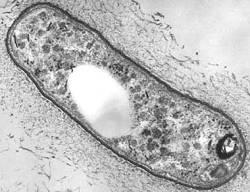
\includegraphics{fractions/bacterie.png}
Figure 2 : Une bactérie en forme de bacille
au microscope électronique

 
Sur la première photo, le virus mesure 1.5 cm et l'échelle est indiquée : 8 mm pour 25 nm
Sur la seconde image, la bactérie mesure 3.4 cm et l'échelle est indiquée : 4.2 cm pour 2 $\mu m$.
Rappel : 1 mm = 1 millimètre = 1'000 $\mu m$ = 1'000 micromètres = 1'000'000 nm = 1'000'000 nanomètres 
\end{enumerate}

\end{exercice}

\section{Corrigés}

\begin{solution}
Simplifier les fractions suivantes :
\begin{multicols}{3}
\begin{enumerate}
\item $\frac{2b}{3a}$
\item $\frac{xy}{b}$
\item $\frac{1}{2(a+3)}$
\item $\frac{a(3{{a}^{2}}+4)}{2{{b}^{2}}}$
\item $a+b$
\item $\frac{4(x+y)}{3(x-y)}$
\item $\frac{x-2}{x+2}$
\item $\frac{1}{8{{a}^{3}}-1}$
\item $\frac{5x+2a}{2ax(5x-2a)}$
\item $\frac{3ax}{2x+5}$
\item $\frac{x-8}{x(x+2)}$
\item $\frac{2(x+3)}{x+7}$
\item $\frac{2x-7}{3(4x-3)}$
\item $\frac{5(2x-1)}{3}$
\item $\frac{{{a}^{2}}+ab+{{b}^{2}}}{a-b}$
\item $x+2$
\item $\frac{2x+1}{x+1}$
\item $\frac{x-7}{{{x}^{2}}+x+1}$
\item $\frac{{{(x+1)}^{2}}}{(x-1)(3{{x}^{2}}+9x+8)}$
\item $\frac{1-x+{{x}^{2}}}{1+x+{{x}^{2}}}$
\item $\frac{2x+1}{2x-1}$
\end{enumerate}
\end{multicols}
\end{solution}


\begin{solution}
Effectuer les opérations suivantes et simplifier :
\begin{multicols}{3}
\begin{enumerate}
\item $\frac{5x}{6}$
\item $\frac{12-x}{6}$
\item $\frac{{{(a+b)}^{2}}}{ab}$
\item $\frac{{{a}^{2}}+{{b}^{2}}}{ab}$
\item $\frac{2x}{(x-6)(x-2)}$
\item $\frac{2xy}{{{x}^{2}}-{{y}^{2}}}$
\item $\frac{2{{x}^{3}}}{1-{{x}^{4}}}$
\item $\frac{2+x}{2-x}$
\item $\frac{-5a}{{{a}^{2}}-1}$
\item 1
\item $\frac{5+2x}{1-{{x}^{2}}}$
\item $\frac{{{y}^{5}}}{{{x}^{6}}-{{y}^{6}}}$
\item $\frac{{{a}^{3}}-{{x}^{3}}}{a}$
\item $\frac{2b}{a+b}$
\item $\frac{ax}{a+x}$
\item $2(x+y)$
\item $\frac{6x}{x+2}$
\item $\frac{1}{1-x}$
\item $\frac{2}{(a+4)(a+2)}$
\item $\frac{2({{a}^{2}}+{{x}^{2}})}{{{a}^{2}}-{{x}^{2}}}$
\item $\frac{ax}{{{x}^{2}}-{{a}^{2}}}$
\item $\frac{5x+9}{{{x}^{2}}-9}$
\item $\frac{3ax}{{{x}^{2}}-4{{a}^{2}}}$
\item $\frac{2(1-x)}{1+x}$
\item $\frac{25x-61}{56}$
\item $\frac{{{a}^{2}}+3{{x}^{2}}}{2ax}$
\item $\frac{{{x}^{3}}+{{y}^{3}}}{{{x}^{2}}{{y}^{3}}}$
\item $\frac{2}{x+y}$
\item $\frac{1}{3-a}$
\item $\frac{a-b}{a+b}$
\item $\frac{2b}{a-b}$
\item $\frac{2(a+1)}{a-1}$
\item $\frac{{{a}^{2}}}{a+b}$
\item $-\frac{a+b}{b}$
\item $\frac{3{{a}^{2}}{{m}^{2}}}{a+m}$
\end{enumerate}
\end{multicols}
\end{solution}

\begin{solution}
Effectuer les opérations suivantes et simplifier :
\begin{multicols}{2}
\begin{enumerate}
\item $\frac{14{{a}^{2}}-15ab-9{{b}^{2}}}{12({{a}^{2}}-{{b}^{2}})}$
\item 1
\item $\frac{2{{a}^{2}}+{{b}^{2}}}{a-b}$
\item 2
\item $\frac{1}{1-{{a}^{2}}}$
\item $\frac{2x-a}{x+a}$
\item $\frac{12}{2x-3}$
\item $\frac{2bx}{4{{x}^{2}}-1}$
\item $\frac{1}{x+2}$
\item $\frac{4}{(x+1)(x-2)}$
\item $\frac{3}{(x-1)(x-3)}$
\item $0$
\item $\frac{a-x}{a+x}$
\item $0$
\item $\frac{2}{c-a}$
\item $0$
\end{enumerate}
\end{multicols}
\end{solution}

\begin{solution}
Effectuer les multiplications suivantes et simplifier :
\begin{multicols}{3}
\begin{enumerate}
\item $\frac{ab}{20}$
\item $-\frac{a{{x}^{2}}}{9}$
\item $\frac{8{{a}^{2}}}{21x}$
\item $-\frac{{{a}^{3}}}{10}$
\item $\frac{4x}{3}$
\item $\frac{4(x-4y)}{x+y}$
\item $\frac{2-a}{2+a}$
\item $-{{(a+6)}^{2}}$
\item $\frac{{{x}^{2}}+2}{x+2}$
\item $\frac{x-3}{x+1}$
\item $\frac{{{x}^{2}}(x-y)}{{{y}^{2}}}$
\item $\frac{(a+x)(x-y)}{2}$
\item $-\frac{5ab(b-3)}{2c}$
\item $\frac{y}{{{x}^{2}}-{{y}^{2}}}$
\item $\frac{3x+2y}{3x+y}$
\item $5\left( 1-x \right)$
\item $x-1$
\item $3$
\item $1$
\item ${{x}^{2}}+xy+{{y}^{2}}$
\item $(2x+5a)(x-a)$
\item $x+3$
\end{enumerate}
\end{multicols}
\end{solution}

\begin{solution}
Effectuer les divisions suivantes et simplifier :
\begin{multicols}{2}
\begin{enumerate}
\item $x-y$
\item ${{(a-b)}^{2}}$
\item $(a-2)(b-3)$
\item ${{a}^{2}}(2x+3{{a}^{2}})$
\item $\frac{(a+b)(x+y)}{a-b}$
\item $\frac{5(3b+4)}{{{a}^{2}}}$
\item $\frac{{{a}^{2}}-{{x}^{2}}}{ax}$
\item $-\frac{a+x}{ax}$
\item $\frac{{{a}^{3}}-1}{a}$
\item $\frac{x-1}{a}$
\item ${{x}^{2}}-ax+{{a}^{2}}$
\item $\frac{x(x-a)}{a(x+a)}$
\item $\frac{x-3}{x(1-x)}$
\item $\frac{-{{x}^{2}}(2x+3)}{2+x}$
\item $\frac{1}{x}$
\item $\frac{{{a}^{2}}-{{b}^{2}}}{2}$
\end{enumerate}
\end{multicols}
\end{solution}

\begin{solution}
Calcul des proportions
\begin{enumerate}
\item Application en économie

Le pourcentage : un rabais de $20 \%$

\begin{tabular}{|l|l|l|l|l|l|}
\hline
Rabais & 20  & 40  & 4  & 2  & 840  \\ \hline
Prix   & 100 & 200 & 20 & 10 & 4200 \\ \hline
\end{tabular}

Le taux de change : 1 \euro = 1.17 Fr. (le 11.07.2011)

\begin{tabular}{|l|l|l|l|l|l|}
\hline
\euro   & 1.00 & 2.00 & 2.14 & 250.50 & 41.03 \\ \hline
Fr. & 1.17 & 2.34 & 2.50 & 293.09 & 48.00 \\ \hline
\end{tabular}

Le salaire d’un vendeur en fonction du chiffre d’affaire : $2 \%$ de commission

\begin{tabular}{|l|l|l|l|l|l|}
\hline
Ventes  & 10'000.00 & 50'000.00 & 200'000.00 & 1'000.00 & 277'750.00 \\ \hline
Salaire & 200.00    & 1'000.00  & 4'000.00   & 20.00    & 5'555.00   \\ \hline
\end{tabular}

Le taux d’intérêt d’un compte épargne : $1.25 \%$ par année

\begin{tabular}{|l|l|l|l|l|l|}
\hline
Montant  & 100.00 & 12'500.00 & 38'400.00 & 151'000.00 & 98'764.80 \\ \hline
Intérêts & 1.25   & 156.25    & 480.00    & 1'887.50   & 1'234.56  \\ \hline
\end{tabular}

\item Application en politique

Les votations : la proportion de « oui »$=1.083/(1.083+1.395)=43.7\%$. Pour le « non » $= 56.3\%$
 
\item Application en géographie

Échelle : environ 3.3 cm

\begin{tabular}{|l|l|l|}
\hline
Réel  & 25'000.00 & 821.10 \\ \hline
Carte & 1.00      & 0.03   \\ \hline
\end{tabular}

L'évolution démographique de la Suisse.

\begin{tabular}{|l|l|l|l|}
\hline
            & 2008    & 2009    & Variation \\ \hline
Émigration  & 86'100  & 86'000  & 0.116\%   \\ \hline
Immigration & 184'300 & 160'600 & -12.86\%  \\ \hline
\end{tabular}

\item Application en Histoire

Les morts de la Seconde Guerre mondiale

\begin{footnotesize}
\begin{tabular}{|l|l|l|l|l|l|}
\hline
Pays        & Pertes militaires & Pertes civiles & Pertes totales & \begin{tabular}[c]{@{}l@{}}Population totale\\   d'avant-guerre\end{tabular} & Pertes en \% \\ \hline
Pologne     & 120'000           & 5'300'000      & 5'420'000      & 36'133'000                                                                   & 15.00\%      \\ \hline
Yougoslavie & 300'000           & 1'200'000      & 1'500'000      & 15'000'000                                                                   & 10.00\%      \\ \hline
Allemagne   & 4'000'000         & 3'000'000      & 7'000'000      & 58'333'333                                                                   & 12.00\%      \\ \hline
Japon       & 2'700'000         & 300'000        & 3'000'000      & 75'000'000                                                                   & 4.00\%       \\ \hline
Italie      & 300'000           & 100'000        & 400'000        & 40'000'000                                                                   & 1.00\%       \\ \hline
France      & 250'000           & 350'000        & 600'000        & 40'000'000                                                                   & 1.50\%       \\ \hline
Royaume-Uni & 326'000           & 62'000         & 388'000        & 48'500'000                                                                   & 0.80\%       \\ \hline
États-Unis  & 300'000           & -              & 300'000        & 150'000'000                                                                  & 0.20\%       \\ \hline
\end{tabular}
\end{footnotesize}
D'après Marc NOUSCHI, Bilan de la Seconde Guerre mondiale, Le Seuil, 1996.

\item Application en sociologie

En fonction de la classe.

\item Application en biologie

Qu’est-ce qui est plus grand : un virus (type grippe) ou une bactérie (type bacille) ?

\begin{tabular}{|l|l|l|}
\hline
\begin{tabular}[c]
{@{}l@{}}Virus\\   à l’échelle (cm)\end{tabular} & 1.500  & 0.80  \\ \hline
Réel (nm)                                                          & 46.875 & 25.00 \\
\hline
\end{tabular}

\begin{tabular}{|l|l|l|}
\hline
\begin{tabular}[c]{@{}l@{}}Bactérie\\   à l’échelle\end{tabular} & 3.40     & 4.20     \\ \hline
Réel (nm)                                                        & 1’619.04 & 2'000.00 \\ \hline
\end{tabular}

On a donc la bactérie qui est environ 34.5 fois plus grande que le virus.
\end{enumerate}
\end{solution}